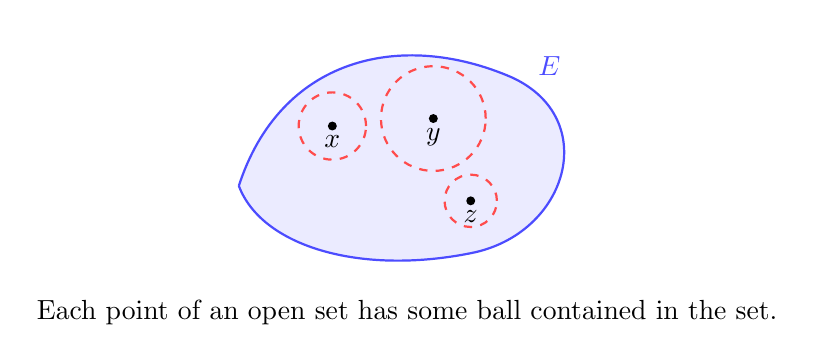
\begin{tikzpicture}[scale=0.95,>=stealth]
  \fill[blue!8]
    (-2.25,-0.45) .. controls (-1.7,1.25) and (-0.1,1.65) .. (1.4,1.0)
    .. controls (2.6,0.45) and (2.15,-1.1) .. (0.85,-1.35)
    .. controls (-0.65,-1.65) and (-1.95,-1.25) .. (-2.25,-0.45);
  \draw[blue!70,thick]
    (-2.25,-0.45) .. controls (-1.7,1.25) and (-0.1,1.65) .. (1.4,1.0)
    .. controls (2.6,0.45) and (2.15,-1.1) .. (0.85,-1.35)
    .. controls (-0.65,-1.65) and (-1.95,-1.25) .. (-2.25,-0.45);
  \node[blue!70] at (1.9,1.15) {\(E\)};

  \foreach \p/\r/\lab in {(-1.0,0.35)/0.45/x,(0.35,0.45)/0.7/y,(0.85,-0.65)/0.35/z}
  {
    \fill[black] \p circle (1.7pt);
    \node[below] at \p {\(\lab\)};
    \draw[red!70,thick,dashed] \p circle (\r);
  }

  \node[align=center] at (0,-2.15)
    {Each point of an open set has some ball contained in the set.};
\end{tikzpicture}
